\documentclass{ps}

\ps{2}
\date{2019 January}
\author{}
\coauthor{}

\begin{document}

\begin{enumerate}
\item The voltage transfer characteristics below are measured for a
  74LS04 operating at \SI{5}{\V}.  Determine \(V_\mathrm{IL}\),
  \(V_\mathrm{IH}\), \(V_\mathrm{OL}\), \(V_\mathrm{OH}\), and the
  high and low noise margins.  Compare your results to the 74LS
  specification in Table eA.2 of the textbook.  Are they within the
  specifications?
  \begin{center}
    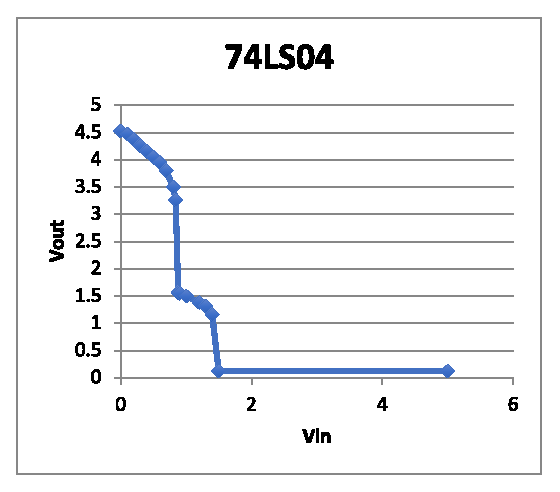
\includegraphics{figures/01.eps}
  \end{center}
  \begin{solution}
  \end{solution}

\item Referring to the logic level specifications in Tables eA.2 and
  eA.3 of the textbook:
  \begin{enumerate}
  \item \label{part:what-could-go-wrong} What could go wrong if a
    74LS04 inverter drives a 74HC08 AND gate?
    \begin{solution}
    \end{solution}
  \item In light of your answer to Part
    \ref{part:what-could-go-wrong}, why does the HCT family exist?
    \begin{solution}
    \end{solution}
  \item
    \begin{enumerate}
    \item Can a 3.3V 74LVC32 gate reliably drive a 5V 74HC00?
      \begin{solution}
      \end{solution}
    \item Can a 3.3V 74LVC32 gate reliably drive a 5V 74HCT00?
      \begin{solution}
      \end{solution}
    \item Can a 74HC00 reliably drive a 3.3V 74LVC32?
      \begin{solution}
      \end{solution}
    \end{enumerate}
  \end{enumerate}

\item Power consumption

  The following circuit turns on an LED when you press one button or
  another but not both.  The circuit operates directly from a 6V
  Ni--MH battery with a \SI{280}{\mA\hour} energy capacity.  The data
  sheet for the 74HC86 XOR gate is attached to the end of this problem
  set.  The circuit is in a hot enclosure that might reach
  \SI{85}{\celsius}.
  \begin{center}
    \begin{tikzpicture}[circuit logic US, font=\small]
      \draw
      (0,0) to[*american voltage source, l_=\SI{6}{\V}] (0,-3) node[sground]{}
      (0,0) to (4,0)
      (1,0) to[*nos] (1,-1) -- (1,-2) to[*american resistor, l^=\(R_1\)] (1,-3) node[sground]{}
      (2,0) to[*nos] (2,-1) -- (2,-2) to[*american resistor, l^=\(R_1\)] (2,-3) node[sground]{}

      (4,-1.5) node[huge circuit symbols, xor gate, inputs=nn](xor){}

      let \p1 = (xor.input 1) in
      (1,\y1) -- +(1,0) to[edge label=\(A\)] (\p1) node[right=2pt]{1}
      let \p1 = (xor.input 2) in
      (2,\y1) to[edge label'=\(B\)] (\p1) node[right=2pt]{2}

      (4,0) -- (xor.north) node[above right]{14}
      (xor.south) node[below right]{7} to[*short] (4,-3) node[sground]{}
      (xor.output) node[left]{3} -- (6,-1.5) node[above]{\(Y\)}
      (5,-1.5) to[*empty diode] (5,-2.25) to[*american resistor, l^=\(R_2\)] (5,-3) node[sground]{};

      \path[logic gate anchors use bounding box]
      (xor.north east) node[above right]{74HC86};
    \end{tikzpicture}

    %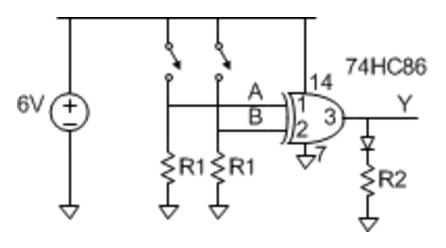
\includegraphics{figures/03.eps}
  \end{center}
  \begin{enumerate}
  \item What is the quiescent power consumption of the XOR gate in the
    hot enclosure?
    \begin{solution}
    \end{solution}
  \item What value of \(R_1\) should you use to minimize power
    consumption when the button is pressed, while still providing a
    valid logic level at the input of the XOR, considering input
    leakage current?
    \begin{solution}
    \end{solution}
  \item What value of \(R_2\) should you use to maximize the
    brightness of the LED without exceeding the \(I_\mathrm{OH}\)
    output current specification?  Assume that the LED has a
    \SI{2}{\V} drop across it when ON.
    \begin{solution}
    \end{solution}
  \item Suppose that both buttons are pressed \SI{99.9}{\percent} of
    the time and that a single button is pressed the remainder of the
    time.  What is the average power consumption?  Be sure to account
    for quiescent consumption of the gate, power dissipated in the
    input resistors, and power delivered to the load.
    \begin{solution}
    \end{solution}
  \item How long will the battery last?
    \begin{solution}
    \end{solution}
  \item If you were willing to violate \(I_\mathrm{OH}\), what is the
    minimum value of \(R_2\) that you could use without risking damage
    to the 74HC86?
    \begin{solution}
    \end{solution}
  \end{enumerate}

\item Sketch a transistor-level implementation of a 3-input NAND gate.
  \begin{solution}
  \end{solution}

\item Give the Boolean equation performed by the following gate.
  \begin{center}
    \begin{tikzpicture}[font=\small]
      \draw
      (0,0)   node[pmos, emptycircle](A1){}
      (0,-1)  node[pmos, emptycircle](B1){}
      (0,-2)  node[pmos, emptycircle](C1){}
      (1,-2)  node[pmos, emptycircle](D1){}

      (1,-3)  node[nmos](D2){}
      (-1,-4) node[nmos](A2){}
      (0,-4)  node[nmos](B2){}
      (1,-4)  node[nmos](C2){}

      (A1.B) node[left]{\(A\)}
      (B1.B) node[left]{\(B\)}
      (C1.B) node[left]{\(C\)}
      (D1.B) node[left]{\(D\)}
      (A2.B) node[left]{\(A\)}
      (B2.B) node[left]{\(B\)}
      (C2.B) node[left]{\(C\)}
      (D2.B) node[left]{\(D\)}
      (A1.C) -- (B1.E) (B1.C) -- (C1.E)
      (A1.E) |- (1,.5) -- (D1.E)
      (C1.C) -- (0,-2.5) to[*short, -*] (1,-2.5) -- (1.5,-2.5) node[right]{\(Y\)}
      (D1.C) -- (D2.C) (D2.E) -- (C2.C)
      (C2.C) -- (A2.C)
      (A2.E) to[*short, -*] (B2.E) node[sground]{} -- (C2.E);
    \end{tikzpicture}

    %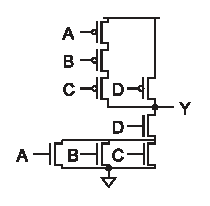
\includegraphics{figures/05.eps}
  \end{center}
  \begin{solution}
  \end{solution}

\item Give a minimal sum of products Boolean equation for the
  following function.  Show how to implement the function with logic
  gates and in Verilog.
  \[
    \begin{array}{ccc|c}
      A&B&C&Y\\\midrule
      0&0&0&1\\
      0&0&1&1\\
      0&1&0&1\\
      0&1&1&0\\
      1&0&0&0\\
      1&0&1&0\\
      1&1&0&0\\
      1&1&1&0\\
    \end{array}
  \]
  \begin{solution}
  \end{solution}

\item Give a minimal sum of products Boolean equation for the
  following function.  Show how to implement the function with logic
  gates and in Verilog.
  \begin{solution}
  \end{solution}

\item Give the minimal sum-of-products equation for the following
  circuit.
  \begin{center}
    \begin{tikzpicture}[circuit logic US, font=\small, huge circuit symbols, scale=.5]
      \matrix[column sep=.5cm, row sep=.5cm]{
        \node[nand gate, inputs=nnn, left](nand-ab){};\\
        \node[nor gate, inputs=nnn, left](nor-bc){};&\node[nand gate, inputs=nnn](nand-all){};\\
        \node[not gate, left](not-a){};\\
      };

      \draw

      let
      \p1 = ($(nand-ab.input 1) + (-1,0)$),
      \p2 = ($(nand-ab.input 1)$),
      \p3 = ($(nand-ab.input 3)$),
      \p4 = ($(nor-bc.input 1)$),
      \p5 = ($(nor-bc.input 3)$),
      \p6 = ($(not-a.input)$)
      in
      (\p2) -- (\x1,\y2) node[left]{\(A\)}
      (\p3) -- (\x1,\y3) node[left]{\(B\)}
      (\p4) -- (\x1,\y4) node[left]{\(B\)}
      (\p5) -- (\x1,\y5) node[left]{\(C\)}
      (\p6) -- (\x1,\y6) node[left]{\(A\)}

      (nand-all.output) -- +(1,0)  node[right]{\(Y\)}

      let
      \p1 = ($(nand-ab.output)!.5!(nand-all.input 1)$),
      \p2 = ($(not-a.output)!.5!(nand-all.input 3)$)
      in
      (nand-ab.output) -| (\p1) |- (nand-all.input 1)
      (not-a.output) -| (\p2) |- (nand-all.input 3)

      (nor-bc.output) -- (nand-all.input 2);
    \end{tikzpicture}

    %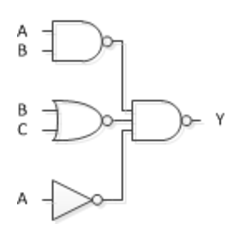
\includegraphics{figures/08.eps}
  \end{center}
  \begin{solution}
  \end{solution}

\item Impact on Society: Integrated circuits have been following
  Moore's Law since 1965, with cost per transistor reducing
  approximately 30\% per year.  This progress is slowing as nanometer
  lithography is becoming extremely expensive.  Supposing cost
  reduction grinds to a halt by 2020, write a thoughtful paragraph
  predicting a significant impact on society caused by the end of
  Moore's Law.
  \begin{solution}
  \end{solution}
\end{enumerate}

How long did you spend on this problem set?  This will not count
toward your grade but will help calibrate the workload.

\end{document}